\documentclass[11pt]{cernrep}
\usepackage{graphicx,epsfig}
\usepackage{color}
\usepackage{fullpage}
\usepackage{mathrsfs}
\usepackage{amsmath, amsthm, amssymb}
\usepackage{amssymb}
\usepackage{verbatim}
\usepackage{hyperref}
\usepackage[compat=1.1.0]{tikz-feynman}

\newcommand{\be}{\begin{equation}}
\newcommand{\ee}{\end{equation}}
\newcommand{\bea}{\begin{eqnarray}}
\newcommand{\eea}{\end{eqnarray}}
\newcommand{\lag}{\mathcal{L}}
\newcommand{\mt}{\mathrm}
\newcommand{\mb}{\mathbf}
\newcommand{\mc}{\mathcal}
\newcommand{\df}{\dfrac}
\newcommand{\miss}{\hspace{-0.2cm} /}
\newcommand{\slashed}{\hspace{-0.3cm} /}
\newcommand{\sv}{\langle\sigma v\rangle}
\usepackage[makeroom]{cancel}

% %%%%%%%%%%%%%% Begin Commands %%%%%%%%%%%%%%%%%%%%%%%%%%%%%%%%%%%%%%%%%%

%% Latin
\def\ie{{\it i.e.}}

%% environments
\def\bsp#1\esp{\begin{split}#1\end{split}}
\def\bpm{\begin{pmatrix}}
\def\epm{\end{pmatrix}}

%% Physics symbols
\def\lag{{\cal L}}
\def\sss{\scriptscriptstyle}
\def\as{\alpha_{\sss s}}
\def\gs{g_{\sss s}}
\def\gL{g_{\sss w}}
\def\gY{g_{\sss Y}}
\def\gF{G_{\sss F}}
\def\tw{\theta_{\sss W}}
\def\ydm{y_{\sss \chi}}
\def\dR{d_{\sss R}}
\def\eR{\ell_{\sss R}}
\def\Ll{L_{\sss L}}
\def\QL{Q_{\sss L}}
\def\QLbar{\bar Q_{\sss L}}
\def\uR{u_{\sss R}}
\def\uRbar{{\bar u}_{\sss R}}

% Tools
\newcommand{\ch}{{\sc\small CalcHep}}
\newcommand{\fa}{{\sc\small FeynArts}}
\newcommand{\fr}{{\sc \small FeynRules}}
\newcommand{\ma}{{\sc\small MadAnalysis}~5}
\newcommand{\maddm}{{\sc\small MadDM}}
\newcommand{\mg}{{\sc\small MG5\_aMC}}
\newcommand{\micromegas}{{\sc\small MicrOMEGAs}}
\newcommand{\mthmtc}{{\sc\small Mathematica}}
\newcommand{\nloct}{{\sc\small NLOCT}}
\def\lqdm{{\tt LQDM}}



\newcommand{\nn}{\nonumber}
\def\ltap{\ \raise.3ex\hbox{$<$\kern-.75em\lower1ex\hbox{$\sim$}}\ }
\def\gtap{\ \raise.3ex\hbox{$>$\kern-.75em\lower1ex\hbox{$\sim$}}\ }
\def\CO{{\cal O}}
\def\CL{{\cal L}}
\def\CM{{\cal M}}
\def\tr{{\rm\ Tr}}
\def\CO{{\cal O}}
\def\CL{{\cal L}}
\def\CM{{\cal M}}
\def\mpl{M_{\rm Pl}}
\newcommand{\bel}[1]{\be\label{#1}}
\def\al{\alpha}
\def\bt{\beta}
\def\eps{\epsilon}
\def\eg{{\it e.g.}}
\def\ie{{\it i.e.}}
\def\mn{{\mu\nu}}
\newcommand{\rep}[1]{{\bf #1}}
\def\bsp#1\esp{\begin{split}#1\end{split}} 
\def\bea{\begin{eqnarray}}
\def\eea{\end{eqnarray}}
\newcommand{\eref}[1]{(\ref{#1})}
\newcommand{\Eref}[1]{Eq.~(\ref{#1})}
\newcommand{\Erefs}[1]{Eqs.~(\ref{#1})}
\newcommand{\gsim}{ \mathop{}_{\textstyle \sim}^{\textstyle >} }
\newcommand{\lsim}{ \mathop{}_{\textstyle \sim}^{\textstyle <} }
\newcommand{\vev}[1]{ \left\langle {#1} \right\rangle }
\newcommand{\bra}[1]{ \langle {#1} | }
\newcommand{\ket}[1]{ | {#1} \rangle }
\newcommand{\fb}{\,{\rm fb}^{-1}}
\newcommand{\ev}{{\rm eV}}
\newcommand{\kev}{{\rm keV}}
\newcommand{\Mev}{{\rm MeV}}
\newcommand{\gev}{{\rm GeV}}
\newcommand{\tev}{{\rm TeV}}
\newcommand{\mev}{{\rm MeV}}
\newcommand{\meV}{{\rm meV}}
\newcommand{\mnu}{\ensuremath{m_\nu}}
\newcommand{\nnu}{\ensuremath{n_\nu}}
\newcommand{\mlr}{\ensuremath{m_{lr}}}
\newcommand{\acc}{\ensuremath{{\cal A}}}
\newcommand{\disc}[1]{{\bf #1}} 
\newcommand{\mh}{{m_h}}
\newcommand{\hb}{{\cal \bar H}}
\def\draftnote#1{{\bf #1}}
\def\mysection#1{{{\bf #1}.~}}
\newcommand{\vckm}{V_{\rm CKM}}
\newcommand{\BR}{{\rm BR}}
\newcommand{\abs}[1]{\left\lvert#1\right\rvert}
\newcommand{\cO}{\mathcal{O}}
\newcommand{\hc}{\rm h.c.}
\definecolor{red1}{cmyk}{0,1,1,0.3}
\newcommand{\redc}[1]{{\color{red1} #1}}

\newcommand{\gSM}{{g_{\rm \scriptscriptstyle SM}}}
\newcommand{\gDM}{{g_{\rm \scriptscriptstyle DM}}}
\newcommand{\mDM}{{m_{\rm \scriptscriptstyle DM}}}
\newcommand{\Mmed}{{M_{\rm med}}}
\newcommand{\Qtr}{{Q_{\rm tr}}}
\newcommand{\sigmaSI}{{\sigma_{\rm \scriptscriptstyle SI}}}
\newcommand{\lmi}{{\lambda_{\rm \scriptscriptstyle mi}}}

\newcommand{\rhochistar}{{\rho_{\chi^*}}}
\newcommand{\rsol}{{r_{\odot}}}
\newcommand{\soldist}{{R_{\odot}}}
\newcommand{\Rss}{{R_{\rm \scriptscriptstyle ss}}}
\newcommand{\eq}[1]{Eq.~(\ref{#1})}

% comments commands
\newcommand{\BZ}[1]{\textbf{\textcolor{blue}{BZ: #1}}}
\def\JZ#1{{\bf  \textcolor{red}{[JZ: {#1}]}}}
\newcommand{\com}[1]{\emph{\color{red}[#1]}}  	% Comments

% definition of flavor anomalies (works in both text mode and math mode)
\def\RD{\ifmmode R_{D^{(*)}} \else $R_{D^{(*)}}$ \fi}
\def\RK{\ifmmode R_{K^{(*)}} \else $R_{K^{(*)}}$ \fi}


\bibliographystyle{lesHouches}
\begin{document}


\title{A common solution to $R_D$ anomalies and Dark Matter}

\author{G. B\'elanger$^1$, J. Bernigaud$^{2,3,4}$, A. Bharucha$^5$, B. Fuks$^6$, J. Heisig$^7$, A. Jueid$^1$, A. Goudelis$^6$, A. Lessa$^8$, D. Marzocca$^{9}$, M. Nardecchia$^{10}$, G. Polesello$^{11}$, P. Pani$^{12}$, D. Sengupta$^{14}$ and J. Zurita$^{3,4}$. }

\institute{$^1$LAPTh, Univ. Grenoble Alpes, USMB, CNRS, LAPTh, 74940 Annecy, France,
\\$^2$ Univ. Grenoble Alpes, Univ. Savoie Mont Blanc, CNRS, LAPTh, 9 Chemin de Bellevue,
F-74000 Annecy, France,
\\$^{3}$ Institute for Nuclear Physics (IKP), KIT Karlsruhe Institute of Technology, 
Hermann-von-Helmholtz-Platz 1, D-76344 Eggenstein-Leopoldshafen, Germany
\\$^{4}$Institute for Theoretical Particle Physics (TTP), Karlsruhe Institute of Technology, 
Engesserstra{\ss} e 7, D-76128 Karlsruhe, Germany
\\$^5$ Laboratoire d'Annecy-le-Vieux de Physique Theorique LAPTh,
CNRS ? USMB, BP 110 Annecy-le-Vieux, F-74941 Annecy, France,
\\$^6$  LPTHE, UMR 7589 - CNRS and Sorbonne Universit\'e, 75252 Paris Cedex, France and Sorbonne Universit\'es, Institut Lagrange de Paris (ILP), 98 bis Boulevard Arago, 75014 Paris, France,
\\$^7$ Centre for Cosmology, Particle Physics and Phenomenology (CP3), Universit\'e catholique de Louvain, Chemin du Cyclotron 2, B-1348 Louvain-la-Neuve, Belgium
\\$^8$ Centro de Ci$\hat{e}$ncias Naturais e Humanas, Universidade Federal do ABC, Santo Andr\'e, 09210-580 SP, Brazil,
\\$^9$ INFN Sezione di Trieste, via Bonomea 265, 34136 Trieste, Italy 
\\$^{10}$ Sapienza - Universita di Roma, Piazzale Aldo Moro 2, 00185, Roma, Italy,
\\$^{11}$ INFN, Sezione di Pavia, Via Bassi 6, 27100 Pavia, Italy,
\\$^{12}$ Deutsches Elektronen Synchrotron, DESY, 15738 Zeuthen, Germany
\\$^{13}$ Department of Physics and Astronomy, 9500 Gilman Drive, University of California, San Diego.}

\maketitle

\begin{abstract}
The anomalies observed by LHCb in flavor observables suggest the breakdown of lepton flavor universality. We study how a vanilla leptoquark solution to the \RD anomalies can also explain the measured relic abundance, if the leptoquark mediates between the visible sector and the dark sector. We find that [something awesome].
\end{abstract}

\section{INTRODUCTION}
The current LHC dataset has not shown any significant deviation from the SM expectations, except for the \RK~\cite{Aaij:2017vbb,Aaij:2019wad} and \RD~\cite{Aaij:2015yra,Aaij:2017uff,Aaij:2017deq} anomalies. While many models have been considered to explain these observations, the consensus is that two classes of models can accommodate these results: leptoquarks and Z' models (for a recent review see e.g~\cite{Blanke:2019pek} and references therein). It is thus interesting to consider the interplay between these solutions and dark matter (DM), which essentially requires to add an additional decay of the leptoquark into the dark sector, studied previously in~\cite{Queiroz:2014pra,Baker:2015qna}. As this will reduce the visible decays of the leptoquarks, this naively allows to lower the current expectation of $m_{LQ} \gtrsim 1~\rm{TeV}$ with ${\cal O} (1) $ couplings, thus opening up novel parameter space and increasing the opportunities to probe this model at the LHC in the near future.

For our study we built a simplified model featuring the minimal ingredients to explain the charged current flavor anomalies \RD  and dark matter simultaneously, limiting ourselves to the couplings strictly necessary to explain the anomaly. We study how the different phenomenological constrains affect the parameter space: LHC searches for leptoquarks and dark matter, relic density and direct detection. We pay particular attention to the existing CMS search for a resonant leptoquark plus mssing energy: while this search might not alway be the golden channel for discovery, its importance lies in the fact that this is indeed probing the $\RD$-DM connection (RDM).

\section{THE MODEL}
\label{sec:model}
\JZ{Text taken from Benj, except for last paragraph.}

We consider a simplified model in which we supplement the Standard Model by one
scalar leptoquark field $S_1$ and two extra fermionic fields, a Majorana
fermion  $\chi_0$ and a Dirac fermion $\chi_1$. The $S_1$ and $\chi_1$ fields
are electrically-charged coloured weak singlets lying in the
$({\bf 3}, {\bf 1})_{-1/3}$ representation of the Standard Model gauge group. In
contrast, $\chi_0$ is a dark matter candidate and therefore a non-coloured
electroweak singlet. In our \fr\ implementation, we consider all potential
interactions of the new sector with the Standard Model sector, the corresponding
Lagrangian being written as
\be\bsp
 \lag = &\ \lag_{\rm SM} + \lag_{\rm kin}
   + \bigg[
    {\bf \lambda_{\sss R}}\ \uRbar^c\ \eR^{\phantom{c}} \ S_1^\dag
  + {\bf \lambda_{\sss L}}\ \QLbar^c \!\cdot\! \Ll^{\phantom{c}} \ S_1^\dag
  + \ydm \bar\chi_1\chi_0 S_1
   + {\rm h.c.} \bigg]\ .
\esp\label{eq:lag}\ee
In this expression, all flavour indices are understood for simplicity and the
dot stands for the $SU(2)$-invariant product of two fields lying in its
fundamental representation. In addition,
$\lag_{\rm SM}$ is the Standard Model Lagrangian and $\lag_{\rm kin}$ contains
gauge-invariant kinetic and mass terms for all new fields, the $\chi_1$ state
being assumed vector-like. The $\QL$ and $\Ll$ spinors stand for the $SU(2)_L$
doublets of left-handed quarks and leptons respectively, whilst $\uR$ and $\eR$
stand for the $SU(2)_L$ singlets of right-handed down-type quarks and charged
leptons, respectively. As can be derived from the omitted flavour structure, the
${\bf \lambda_{\sss L}}$ and ${\bf \lambda_{\sss R}}$ couplings are $3\times 3$
matrices in the flavour space, that are considered real in the following.
Moreover, in our
conventions, the first index $i$ of any $\lambda_{ij}$ element refers to the
quark generation whilst the second one $j$ refers to the lepton generation.


The field content of the new physics sector of our simplified model is
presented in table~\ref{tab:fields}, together with the corresponding
representation under the gauge and Poincar\'e groups, the potential Majorana
nature of the different particles, the adopted symbol in the \fr\
implementation and the PDG identifier that has been chosen for
each particle. The new physics coupling parameters are collected in
table~\ref{tab:params}, in which we additionally include the name used in the
\fr\ model and the Les Houches blocks in which the numerical values of
the different parameters can be changed by the user when running tools like
\mg\ or \micromegas.

\begin{table}[h]
\renewcommand{\arraystretch}{1.4}
\setlength\tabcolsep{8pt}
\begin{tabular}{c c c c c c}
  Field & Spin & Repr. & Self-conj. & \fr\ name & PDG code\\
  \hline\hline
  $S_1$    & 0   & $({\bf 3}, {\bf 1})_{-1/3}$ & no  & {\tt LQ} & 42\\
  $\chi_0$ & 1/2 & $({\bf 1}, {\bf 1})_0$      & yes & {\tt chi0} & 5000521\\
  $\chi_1$ & 1/2 & $({\bf 3}, {\bf 1})_{-1/3}$ & no  & {\tt chi1} & 5000522\\
\end{tabular}
\caption{\it New particles supplementing the Standard Model, given
  together with the representations under $SU(3)_c\times SU(2)_L \times U(1)_Y$.
  We additionally indicate whether the particles are Majorana particles,
  their name in the \fr\ implementation and the associated Particle Data Group
  (PDG) identifier.}
\label{tab:fields}
\end{table}

\begin{table}[h]
\renewcommand{\arraystretch}{1.4}
\setlength\tabcolsep{15pt}
\begin{tabular}{c c c c}
  Coupling & \fr\ name & Les Houches block\\
  \hline\hline
  $(\lambda_{\sss L})_{ij}$ & {\tt lamL} & {\tt LQLAML}\\
  $(\lambda_{\sss R})_{ij}$ & {\tt lamR} & {\tt LQLAMR}\\
  $\ydm$ & {\tt yDM} & {\tt DMINPUTS}\\
\end{tabular}
\caption{\it Couplings of the new particles, given together with the associated
  \fr\ symbol and the Les Houches block of the parameter card.}
\label{tab:params}
\end{table}
In a nutshell, our model needs three new masses and several new couplings.The $R_D$ anomalies can be solved with only $(\lambda_{\sss L})_{33} \equiv \lambda_L$~\footnote{As the neutrino flavor is not tagged, in principle the second index is not constrained. For simplicity we restrict it here to the third generation.} and $(\lambda_{\sss R})_{23} \equiv \lambda_R$. Finally, the dark matter phenomenology requires the coupling $\ydm$. Hence these 6 parameters span our parameter space. In what follows we will study how the flavor anomalies, dark matter phenomenology and collider searches constrain this parameter space, showing the currently allowed parameter space and commenting on the future prospects. 


\section{LEPTOQUARK SOLUTIONS TO  $R_D$ ANOMALIES}

As mentioned in the previous chapter, a minimal solution of the $R(D)$ anomalies can be obtained with just a left-handed (33) and a right-handed (32) couplings to $S_1$. We note that the $33$ coupling is forced to be left-handed due to the presence of the neutrino~\footnote{Alternatively one could consider a right handed by explicitly introducing a right-handed neutrino that could serve as a dark matter candidate, see e.g~\cite{Azatov:2018kzb}.}. The choice of having a right-handed coupling for the $32$ interaction is due to the large contributions that a left-handed coupling would generate to the $B \to X_s \nu \nu$ process, which in turn would require the addition of another leptoquark state \cite{Crivellin:2017zlb,Buttazzo:2017ixm,Marzocca:2018wcf,Crivellin:2019dwb}.
%
We perform a global fit of the model with the two couplings $(\lambda_{\sss L})_{33}$ and $(\lambda_{\sss R})_{23}$ as free parameters. The relevant observables included in the fit are: $R_D$, $R_D^*$, $\text{Br}(B_c \to \tau \nu)$, deviations in the $Z$ couplings to $\tau_L$ and $\tau_R$, effective number of neutrinos from $Z$ decays, lepton flavour universality test in $\tau$ decays. For more details on this fit see e.g.~\cite{Buttazzo:2017ixm,Marzocca:2018wcf,Azatov:2018kzb}. A contribution to $D^0 - \bar{D}^0$ mixing is generated at one loop, but it is strongly CKM-suppressed and does not provide a strong constraint.
The results of a scan in the two parameters of the model, for $m_{S_1} = 1.5 \text{TeV}$, where all points are within $1\sigma$ of the best-fit point, is shown in the plane of the $R_D$ and $R_D^*$ anomalies in the left panel of figure~\ref{fig:FlaFit}. The corresponding preferred region in the two couplings is presented in the right panel of figure~\ref{fig:FlaFit}.\footnote{Defining $x= \lambda_L / m_{S_1}$ and $y= \lambda_R / m_{S_1}$ we have that the anomalies would scale with the product $xy$. Other constraints scale instead like $x^2$ or $y^2$.}

%%%%%%%%%%
 \begin{figure}[!htp]
  \centering
  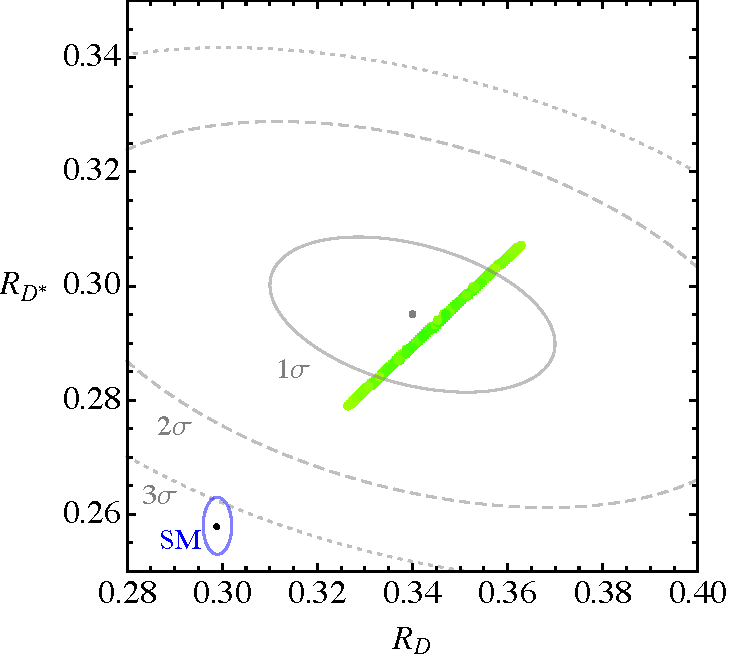
\includegraphics[width=0.49\textwidth]{./figures/FlavorFit_RDRDst.pdf} 
  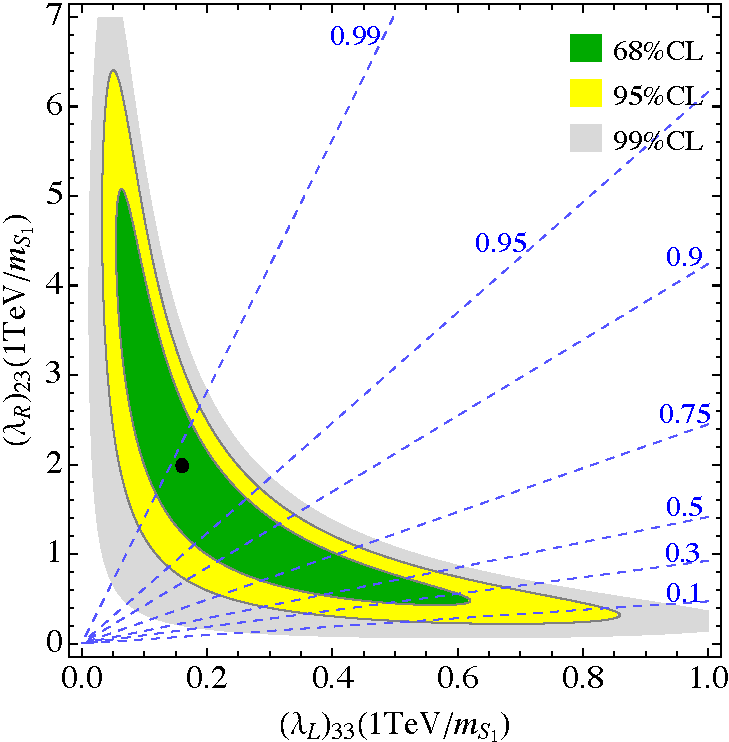
\includegraphics[width=0.44\textwidth]{./figures/FlavorFit_S1.pdf} 
  \caption{\it Left: flavor fit to the charged current anomalies for $m_{S_1}=1.5$ TeV ($1\sigma$ region). The gray lines represent the present status in the measurements of the two observables, compared with the SM point (blue point and contour). Right: Viable parameter space from the fit of flavor and precision observables as function of $\lambda / m_{S_1}$. Blue dashed lines are iso-lines of the branching ratio $B(S_1 \to c_R \tau_R)$ assuming $y_\chi \ll (\lambda_L)_{33}, (\lambda_R)_{23}$ and $m_{S_1} \gg m_t$. The black dot represents the best-fit point.}
\label{fig:FlaFit}
\end{figure}
%%%%%%%%%%%





From the figure we can establish two working points. We pick the first one to obtain the lowest possible  $BR (S_1 \to c \tau)$, which corresponds to  $(x,y) = (0.6,0.5)$. For the second one we do not want to pick extreme values of $\lambda_R$, as we could run into the regime of a ``fat" leptoquark, namely having a width comparable to its mass. So we restrict ourselves to the best fit point  $(0.16,2.0)$ that already gives a negligible branching fraction into the third generation states. We thus use these working points to generate concrete benchmarks by picking two values for the leptoquark mass: $m_{S_1}= 500$ GeV and $m_{S_1}= 1000$ GeV. We show the corresponding values of the couplings and branching ratios in Table~\ref{tab:benchmark_points}, where we have assumed a negligible coupling of $S_1$ to the dark sector. We note that the solution of the $\RD$ anomalies, being an off-shell interference with the SM amplitude, will not be affected by diluting the leptoquark visible decays, but it would rather loose the constraints coming from direct searches of $S_1$, which we discuss in detail in Section~\ref{sec:lhc}.
\begin{table}[]
\begin{tabular}{lllllll}
$m_{S_1}$ {[}GeV{]} & $\lambda_L$ & $\lambda_R$ & $BR(S_1 \to b \nu)$ & $BR(S_1 \to t \tau)$ & $BR(S_1 \to c \tau)$ & $\Gamma(S_1)/m_{S_1}$ \\
\hline 
500                 & 0.30        & 0.25        & 0.4049              & 0.3139               & 0.2812               & 4.42E-3               \\
1000                & 0.6         & 0.5         & 0.3794              & 0.3571               & 0.2635               & 1.89E-2               \\
500                 & 0.08        & 1.0         & 0.0063              & 0.0049               & 0.9887               & 3.4E-2                \\
1000                & 0.16        & 2.0         & 0.0063              & 0.0059               & 0.9877               & 8.06E-2              
\end{tabular}
\caption{Benchmark points compatible with the flavour anomalies. Here we have assumed negligible decays into the dark sector. Note the wide range of possibilities for the $c-\tau$ channel (from 25 \% to roughly 100\%) while the b and top decays have an upper bound of about 40 and 30 \% respectively, and can actually become at the sub-percent level.}
\label{tab:benchmark_points}
\end{table}

Having established the parameter space in the $\lambda_L, \lambda_R$ and $m_{S_1}$ we will focus in the next section on the constraints given by dark matter observables: relic density, direct detection and indirect detection.




\section{DARK MATTER CONSTRAINTS}

In this section we study how the measured relic density and the null results of direct detection impact on our model. We start by noting that the direct detection rate is suppressed at 1-loop \JZ{draw box diagrams}, however given the current $\sigma_{SI}$ exclusions this suppression might not be enough to discard this observable. For the relic density we consider two distinct scenarios. On one hand we study the (co)-annihilation case, as done in~\cite{Baker:2015qna}, while on the other hand we also consider the conversion-driven freeze-out (CDFO) scenario~\cite{Garny:2017rxs}, also known as co-scattering~\cite{DAgnolo:2017dbv}. The main idea behind this mechanism is that the self-annihilation of the dark matter candidate is negligible: the dark matter abundance arises instead from conversion processes within the dark sector. Hence, this scenario requires small/tiny interactions between the SM and the DM candidate ($y_{DM}$ in our case), thus rendering the $BR(S_1 \to \chi_1 \chi_0)$ negligible. This will thus affect the relevance of the collider signatures, that are discussed in detail in section~\ref{sec:lhc}

\subsection{Direct Detection}
\JZ{Under study by GB, AG, DS, JB}

The scattering of $\chi_0$ on a nucleon proceeds via 1-loop diagrams, which we show in figure~\ref{fig:dd_1loop}. In the first diagram the loop include two leptoquark masses and the $\chi_1$ mass, which are already heavy enough compared with the typical momentum transfer, so that would naively induce a mass suppression. In the second diagram one would have three leptoquark masses and a $\chi_1$ mass, so that would be more suppressed than the diagram with three $\chi_1$ and one $S_1$ in the loop.
\JZ{What follows is highly speculative and must be taken as such, the final answer will come from the explicit calculation of Andreas and Aoife.}
We can obtain a rough estimate of the size of these contributions by first integrating out the $S_1$. We then would end with 
\begin{itemize}
\item a 1-loop bubble with $\chi_1$ and a lepton propagating in the loop and two effective couplings.
\item a \JZ{not sure about this one} tree level diagram with $\chi_0 g \to \chi_0 g$ via a $\chi_1$ exchange.
\item a 1-loop triangle with $\chi_1$ running in the loop and one effective $\chi_1-\chi_1-\chi_0-\chi_0$ vertex.
\end{itemize}
Among the three possibilities, the third one is naively the less suppressed one since it has only one effective coupling less, and the lowest power in $m_{S_1}$.~\footnote{Of course one can also integrate out $\chi_1$ and directly write the $\chi_0 \bar{\chi_0} G^a_{\mu \nu} G^{a \, \mu \nu}$, but then one would lose the explicit couplings and massses}. Hence the diagram scales as 
\be
\frac{1}{4 \pi m_{S_1}} y_{DM}^2 \alpha_s * \frac{8 \pi}{9 \alpha_s} m_P f_{T,G} \sim \frac{0.2}{m_{S_1}} y_{DM}^2 \, ,
\ee 
and thus the suppression is not very high: nowadays 1-loop EW corrections and 1-loop QCD corrections for WIMPS are relevant, and here we are at a similar level. \JZ{Here I tried to conclude that we need the calculation, but once we have the final result we can use this disgression as a ``a posteriori" justification.}
\JZ{end of speculation}

\begin{figure}[!t]
\center
\scalebox{0.95}{
\begin{tikzpicture}
\node at (0,0) {\includegraphics[scale=0.43]{figures/directDetection.eps} };
\node at (-2.6,2.3) {\scalebox{1.3}{$\chi_0$}};
\node at (2.6,2.3) {\scalebox{1.3}{$\chi_0$}};
\node at (0,1.4) {\scalebox{1.3}{$\chi_1$}};
\node at (-1.5,0) {\scalebox{1.3}{$S_1$}};
\node at (1.5,0) {\scalebox{1.3}{$S_1$}};
\node at (-2.4,-2.2) {\scalebox{1.3}{$q$}};
\node at (2.6,-2.2) {\scalebox{1.3}{$q$}};
\node at (0,-1.4) {\scalebox{1.3}{$\ell$}};
\end{tikzpicture}
\begin{tikzpicture}
\node at (0,0) {\includegraphics[scale=0.43]{figures/directDetection.eps} };
\node at (-2.6,2.3) {\scalebox{1.3}{$\chi_0$}};
\node at (2.6,2.3) {\scalebox{1.3}{$\chi_0$}};
\node at (0,1.4) {\scalebox{1.3}{$\chi_1$}};
\node at (-1.5,0) {\scalebox{1.3}{$S_1$}};
\node at (1.5,0) {\scalebox{1.3}{$S_1$}};
\node at (-2.4,-2.2) {\scalebox{1.3}{$g$}};
\node at (2.6,-2.2) {\scalebox{1.3}{$g$}};
\node at (0,-1.4) {\scalebox{1.3}{$S_1$}};
\end{tikzpicture}
\begin{tikzpicture}
\node at (0,0) {\includegraphics[scale=0.43]{figures/directDetection.eps} };
\node at (-2.6,2.3) {\scalebox{1.3}{$\chi_0$}};
\node at (2.6,2.3) {\scalebox{1.3}{$\chi_0$}};
\node at (0,1.4) {\scalebox{1.3}{$S_1$}};
\node at (-1.5,0) {\scalebox{1.3}{$\chi_1$}};
\node at (1.5,0) {\scalebox{1.3}{$\chi_1$}};
\node at (-2.4,-2.2) {\scalebox{1.3}{$g$}};
\node at (2.6,-2.2) {\scalebox{1.3}{$g$}};
\node at (0,-1.4) {\scalebox{1.3}{$\chi_1$}};
\end{tikzpicture}
}
\caption{Feynman diagrams for the direct detection of dark matter in our model at the lowest order in perturbation theory.
\JZ{Need to change some lines for second and third diagram. Please use your imagination}.}
\label{fig:dd_1loop}
\end{figure}
\subsection{Relic Density}

\JZ{Coannihilation done with Micromegas. CDFO: Under study by GB, JH, AL, AG, JB}

Preliminary results using the LQ solution to the flavor anomalies and satisfying the correct relic density are displayed in Fig.~\ref{fig:CDFO_WIMP}.

%%%%%%%%%%%%%%%%%%%%%%%%%%%%%%%%%%%%%%%%%%%%%%%%%%%%%%%%%%%%%%%%%%%%%%%%%%%%%%%%%%%%%%%%%%%%%%%%%%%%%%%%%%%%%%
 \begin{figure}[!htp]
  \centering
  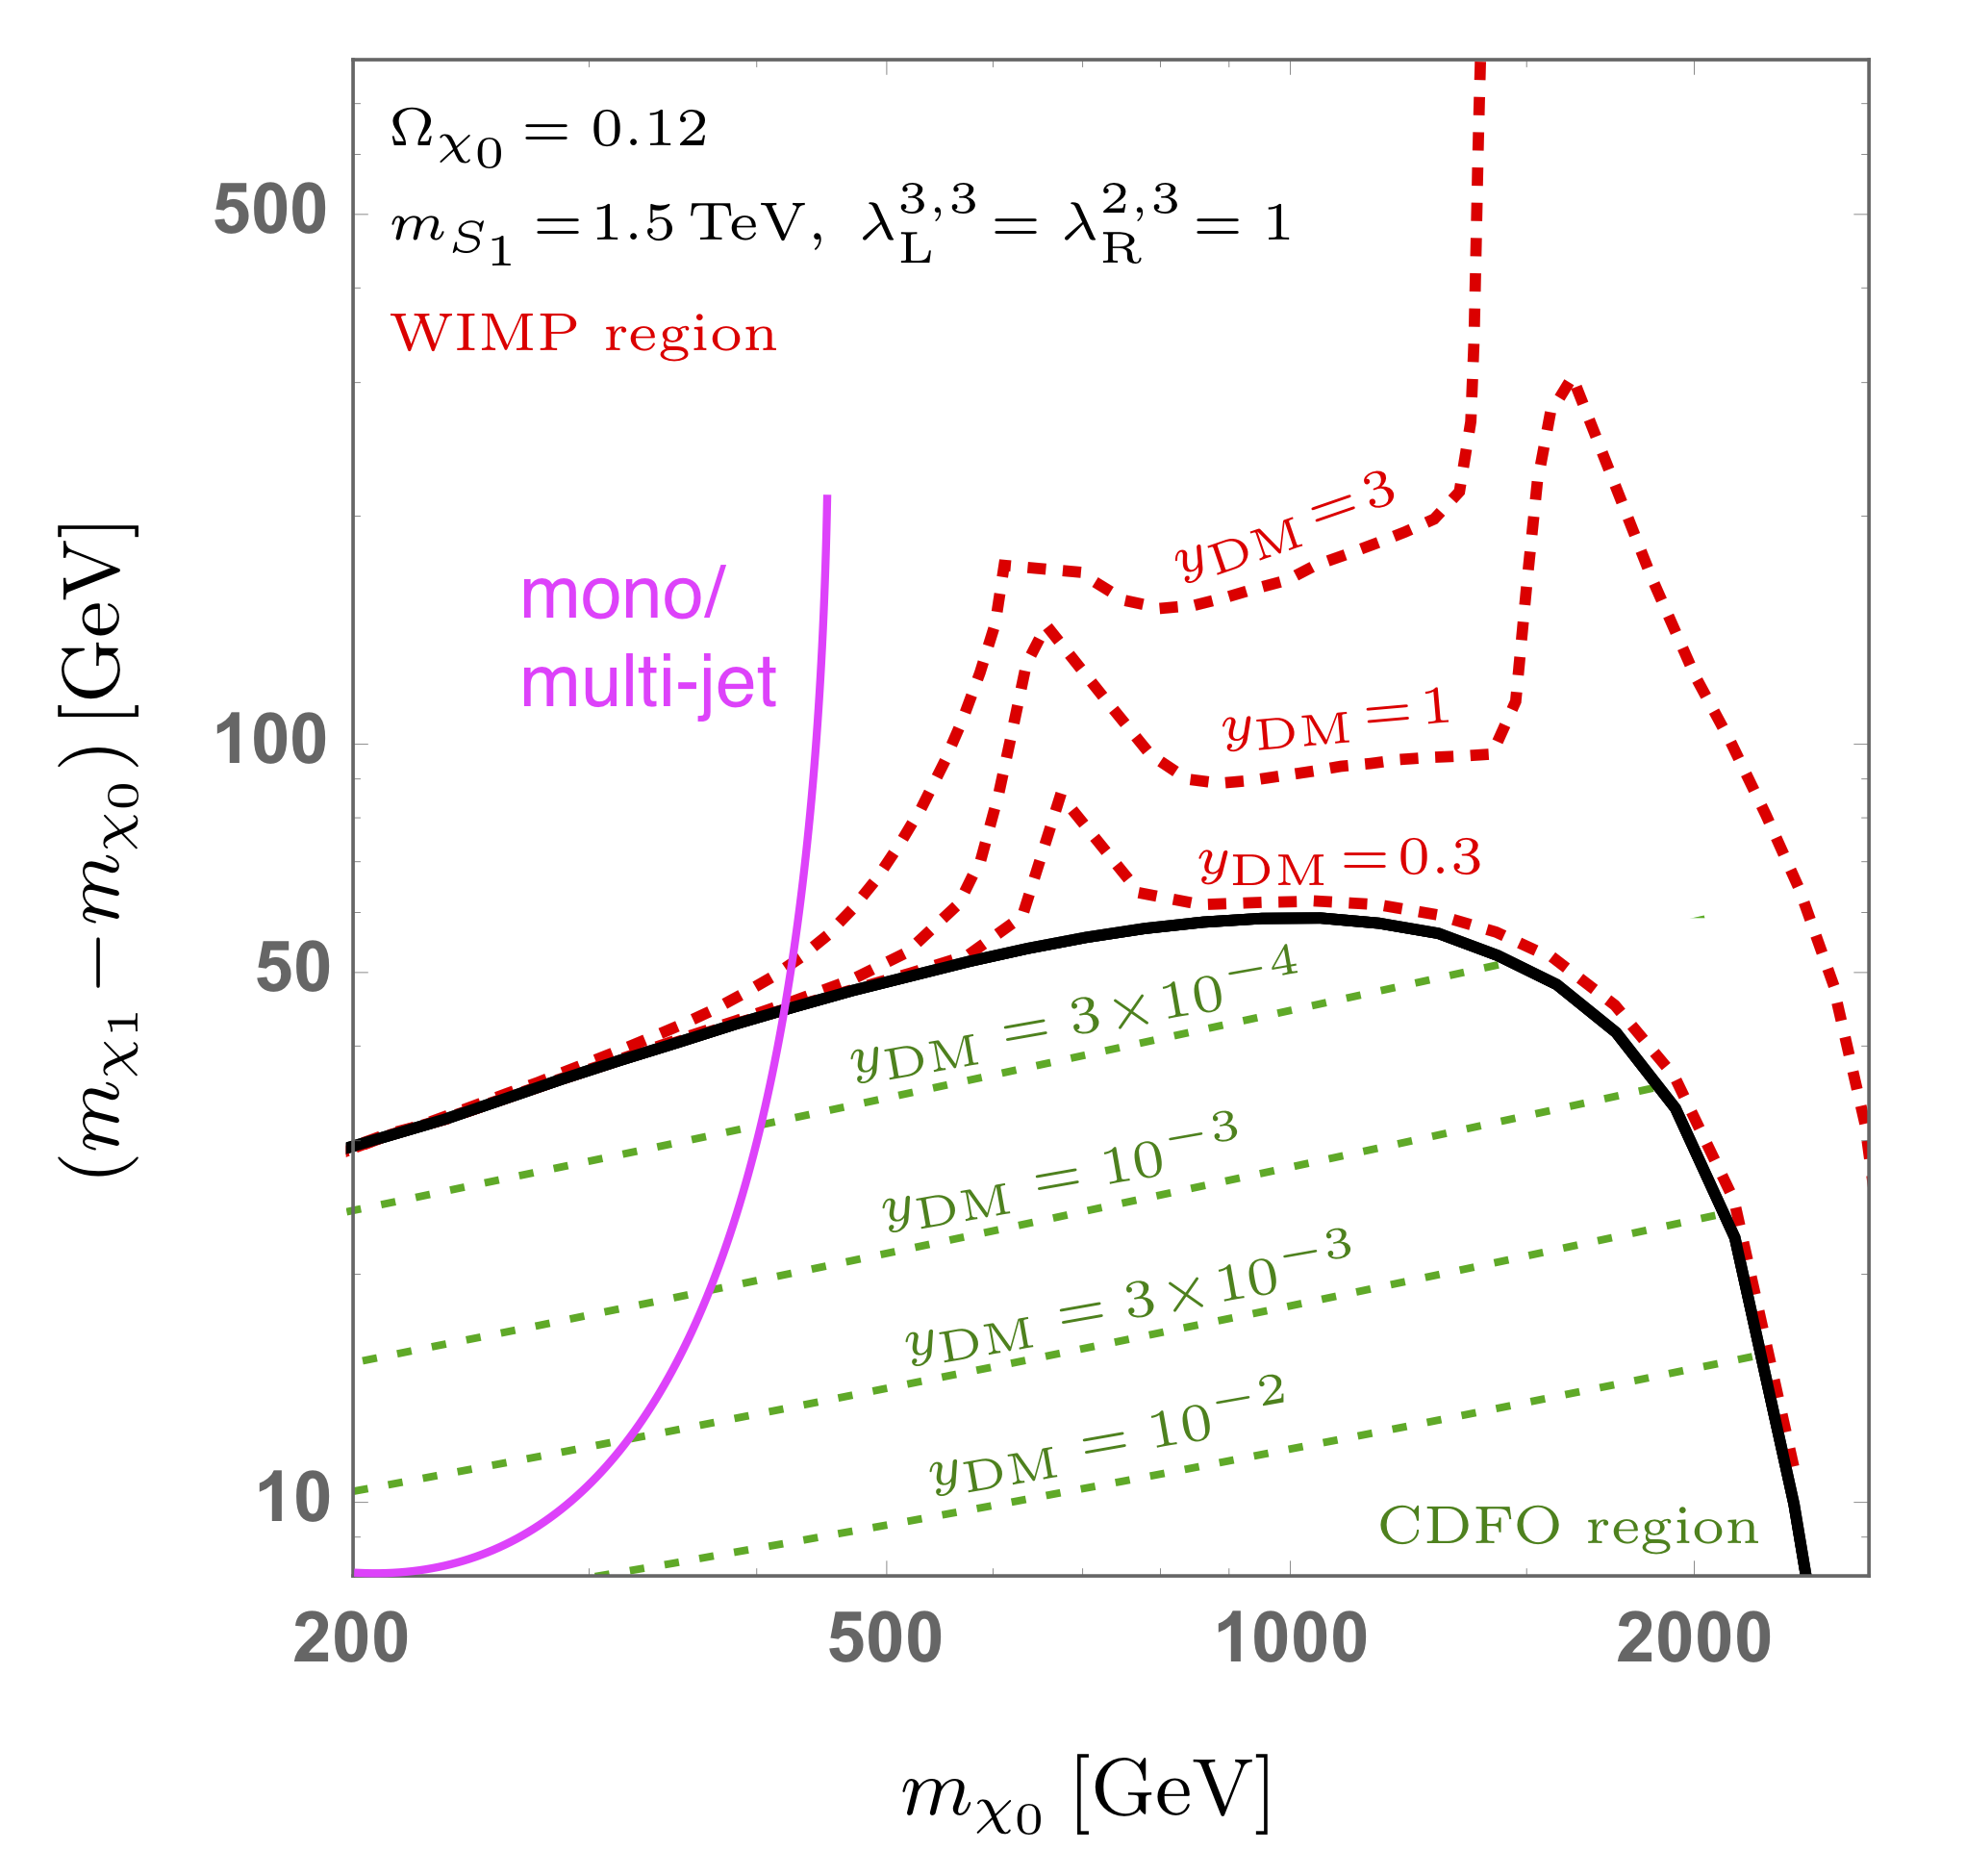
\includegraphics[width=0.5\textwidth]{./figures/CDFO_WIMP_region_toyMJ_v1.png} 
  \caption{\it Parameters space in the $m_{\chi_0} - \Delta = m_{\chi_1} - m_{\chi_0}$ plane satisfying $\Omega h^2 = 0.12$. The solid black line denotes the boundary between the coannihilation (CA) and the conversion-driven freeze-out (CDFO) regimes. The dashed lines also indicate the specific value of $Y_{dm}$. We also overlay a naive hand-waving estimate of the mono-jet reach (see Section~\ref{subsec:mjet}).}
\label{fig:CDFO_WIMP}
\end{figure}
%%%%%%%%%%%%%%%%%%%%%%%%%%%%%%%%%%%%%%%%%%%%%%%%%%%%%%%%%%%%%%%%%%%%%%%%%%%%%%%%%%%%%%%%%%%%%%%%%%%%%%%%%%%%%%



\subsection{Indirect Detection}

\JZ{JH and AG want to write something about it.}

Indirect detection constitutes an important probe of the self-annihilating nature of dark matter. 
In the considered model annihilation today dominantly takes place either via the $2\to2$ process 
$\chi^0 \chi^0 \to S_1 S_1$, if $m_{S_1}< m_{\chi^0}$, or 
via $2\to 4$ or loop-induced $2\to2$ processes otherwise. \com{Right?} 
Figure~\ref{fig:anndiag} shows an exemplary $2\to 4$ annihilation 
diagram. As these processes are suppressed by the off-shell $S_1$ propagator (or loop-suppressed)
we expect small annihilation rates.
In particular, if annihilation during freeze-out proceeds dominantly via $\chi^0 \chi^\pm$ co-annihilation or 
pair-annihilation of $\chi^\pm$, the relic density constraint does not require the dark matter self-annihilation 
rate to be large and hence we expect it to fall below the sensitivity of indirect detection experiments.

In Figure~\ref{fig:IDspec} we show an exemplary gamma-ray and antiproton spectra per annihilation for a benchmark point
with $m_{\chi^0}=150\,$GeV, $m_{\chi^\pm}=600\,$GeV and $m_{S_1}=1\,$TeV. Note that as long as 
$m_{S_1}> m_{\chi^0}$ (and, of course, $m_{\chi^\pm}> m_{\chi^0}$) the masses $m_{S_1}$ and $m_{\chi^\pm}$ 
are not expected to have a significant effect on the shape of the spectrum but mainly change the annihilation cross section,
\emph{i.e.}~the total normalization of the signal.
We also compare the spectra to the ones for annihilation into $b\bar b$ which is an often
quoted reference channel in the literature (choosing the same dark matter mass). 
While the gamma-ray spectrum is very similar to the one for $b\bar b$,
the antiproton spectrum is slightly more peaked. However, it does not exhibit a distinct feature that is expected to 
alter the constraints with respect to the case of $b\bar b$ drastically. Accordingly, we can use the limits on $b\bar b$
for an order-of-magnitude estimate of indirect detection limits in our model and use them to asses their relevance.
\com{Just as a proposal. Needs to be further checked, of course.}


%=====================
%    \                                           |
%      \                                         |
%        \                                       |
\begin{figure}[t]
\centering
\setlength{\unitlength}{1\textwidth}
\begin{picture}(0.975,0.355)
 \put(-0.0055,-0.01){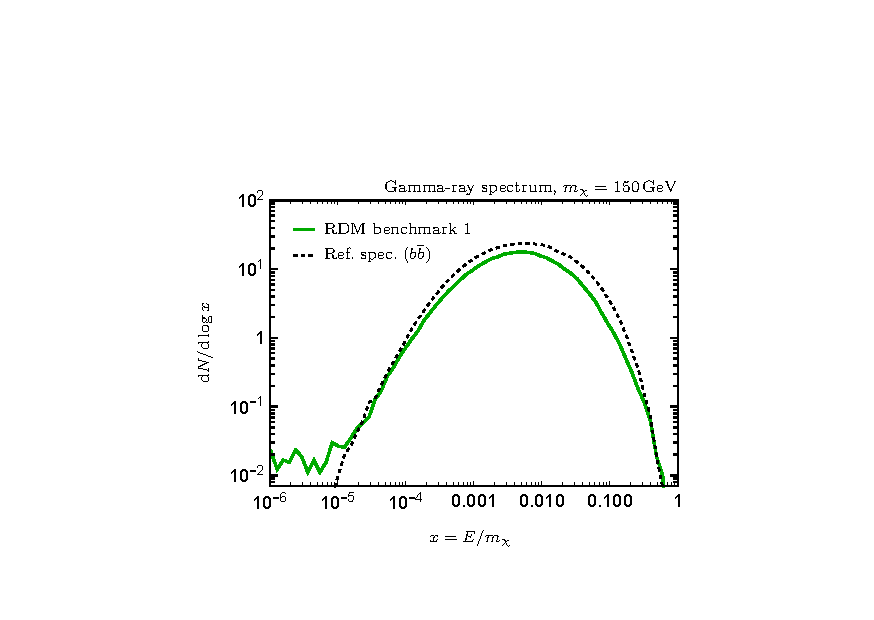
\includegraphics[width=0.48\textwidth, trim= {3.3cm 1.2cm 3cm 2cm}, clip]{figures/plot_gamma_spectra.pdf}}
 \put(0.506,-0.01){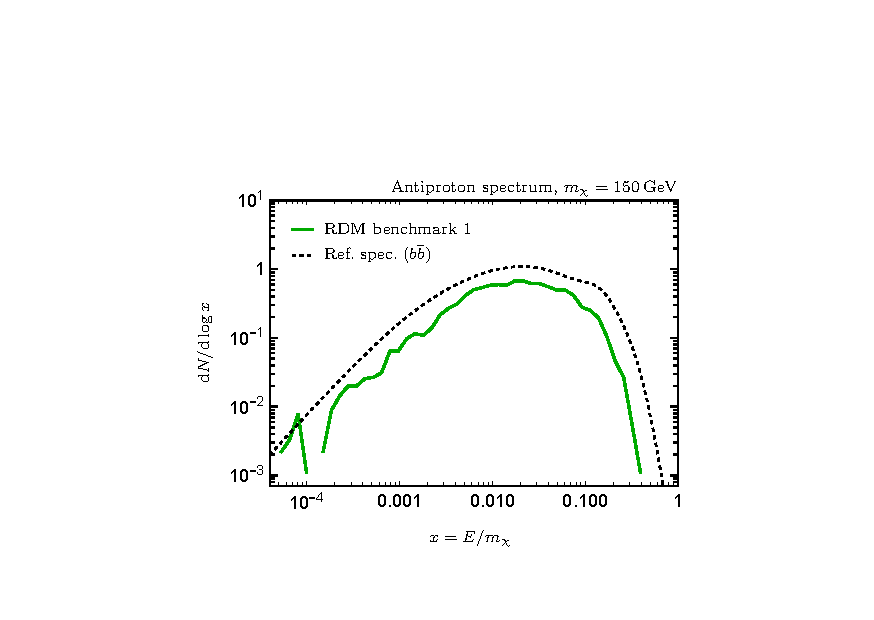
\includegraphics[width=0.48\textwidth, trim= {3.3cm 1.2cm 3cm 2cm}, clip]{figures/plot_pbar_spectra.pdf}}
\end{picture}
\caption{%
Exemplary gamma-ray (left panel) and antiproton spectra (right panel) for dark matter annihilation of the benchmark point
with $m_{\chi^0}=150\,$GeV, $m_{\chi^\pm}=600\,$GeV and $m_{S_1}=1\,$TeV (green curves). For comparison we show 
the corresponding reference spectra for annihilation into $b \bar b$ (black dotted curves).
\label{fig:IDspec}
}
\end{figure}
%                                      \         |
%                                        \       |
%                                          \     |
%=====================


%=====================
%    \                                           |
%      \                                         |
%        \                                       |
\begin{figure}[t]
\centering
\setlength{\unitlength}{1\textwidth}
\begin{picture}(0.975,0.355)
 \put(-0.0055,-0.01){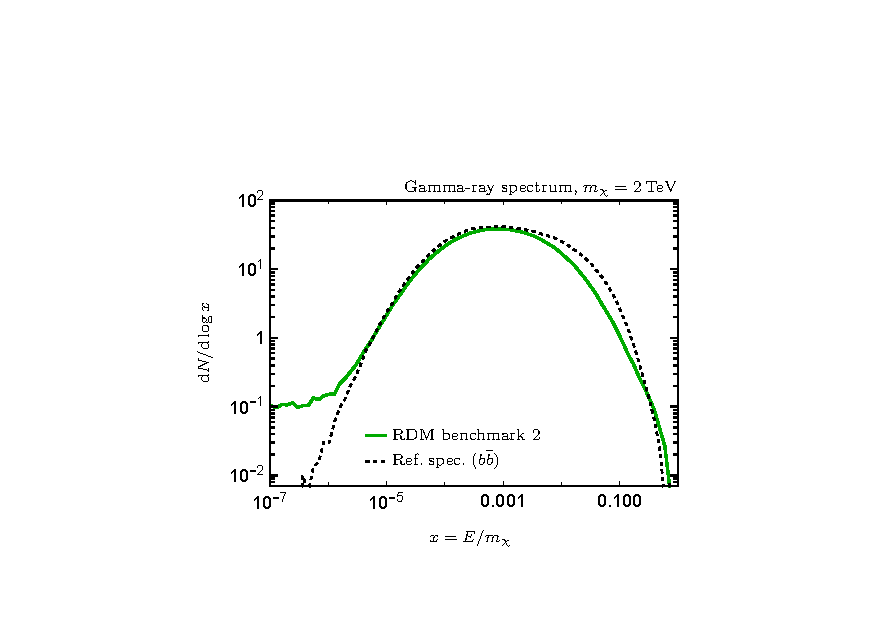
\includegraphics[width=0.48\textwidth, trim= {3.3cm 1.2cm 3cm 2cm}, clip]{figures/plot_gamma_spectra2.pdf}}
 \put(0.506,-0.01){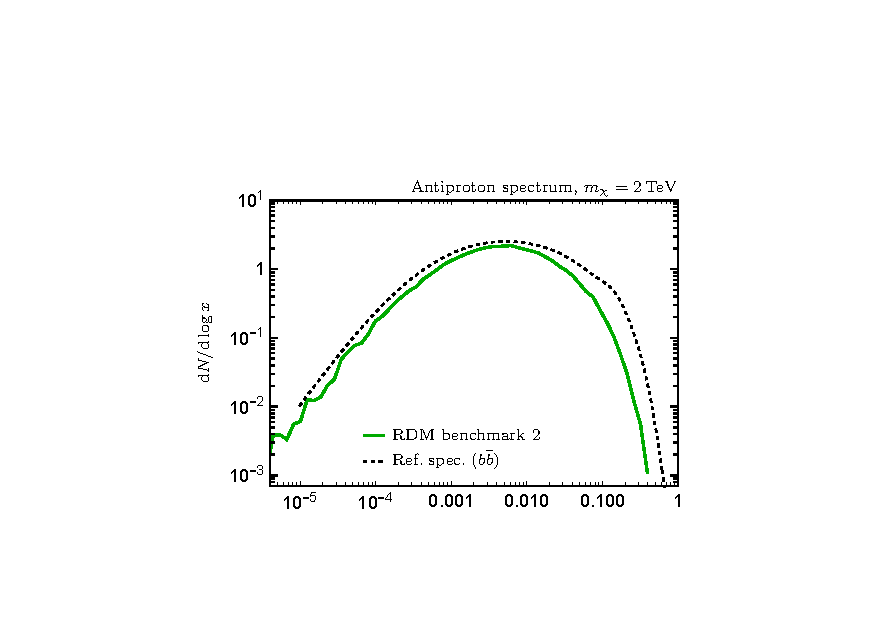
\includegraphics[width=0.48\textwidth, trim= {3.3cm 1.2cm 3cm 2cm}, clip]{figures/plot_pbar_spectra2.pdf}}
\end{picture}
\caption{%
Exemplary gamma-ray (left panel) and antiproton spectra (right panel) for dark matter annihilation of the benchmark point
with $m_{\chi^0}=2\,$TeV, $m_{\chi^\pm}=2.5\,$TeV and $m_{S_1}=1.5\,$TeV (green curves). For comparison we show 
the corresponding reference spectra for annihilation into $b \bar b$ (black dotted curves).
\label{fig:IDspec}
}
\end{figure}
%                                      \         |
%                                        \       |
%                                          \     |
%=====================



%=====================
%    \                                           |
%      \                                         |
%        \                                       |
\begin{figure}[t]
\centering
\setlength{\unitlength}{1\textwidth}
\begin{picture}(0.35,0.26)
 \put(0.00,-0.01){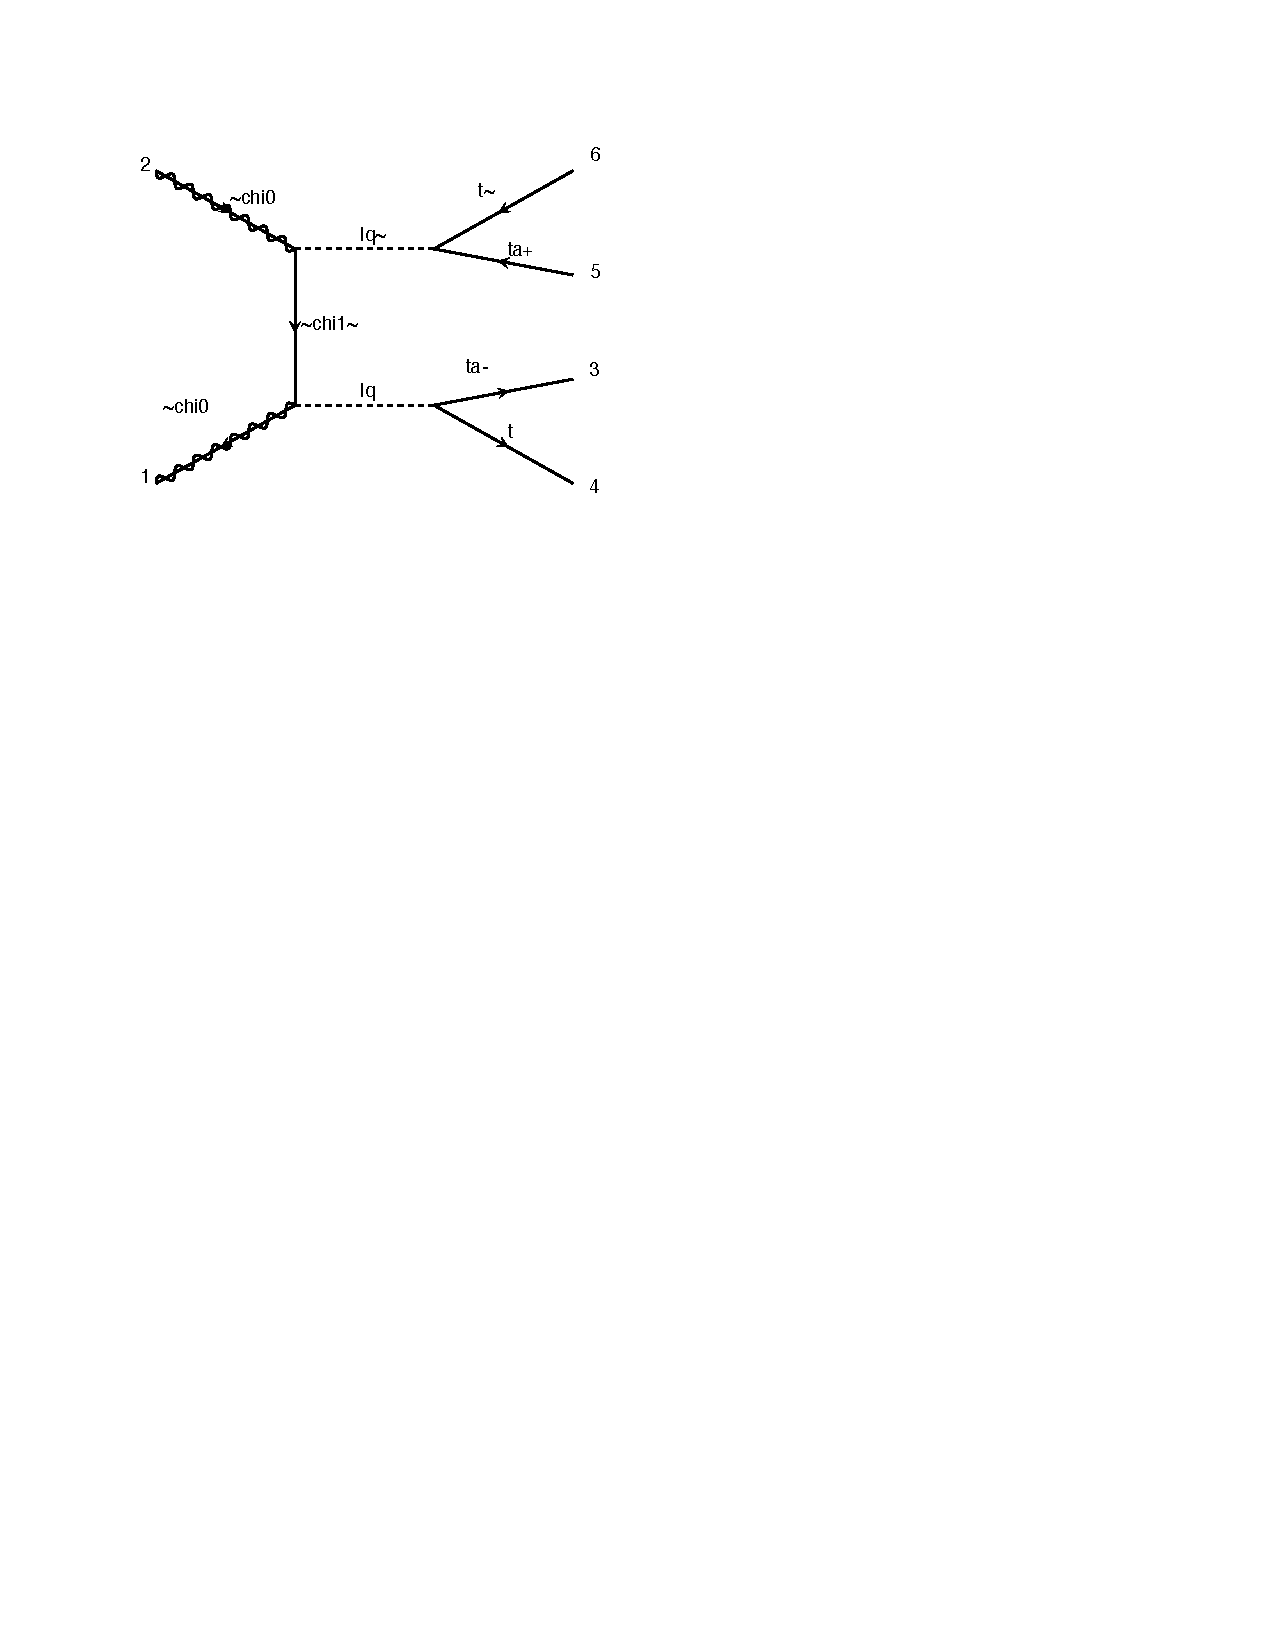
\includegraphics[width=0.33\textwidth]{figures/ann_diag.pdf}}
\end{picture}
\caption{%
Exemplary $2\to4$ dark matter annihilation diagram.
\label{fig:anndiag}
}
\end{figure}
%                                      \         |
%                                        \       |
%                                          \     |
%=====================



\section{LHC CONSTRAINTS}
\label{sec:lhc}
Our model contains three new fields that are probed by several LHC searches, which generically fall into two categories. On one hand, we have direct searches for leptoquarks ($S_1$), both for single and double production. On the other hand we have the full spectrum of missing energy (MET) searches targeting dark matter observables, in our case driven by pair production of $\chi_1$ via gauge interactions . As a hybrid of both categories, the CMS search for leptoquark plus dark matter~\cite{Sirunyan:2018xtm}, inspired by the Coannihilation Codex~\cite{Baker:2015qna}, gives not only interesting constraints on the parameter space, but moreover it would allow to establish the connection between flavor anomalies and dark matter, in a post-discovery scenario. 

In each of the categories described above, we will consider both a) existing searches and b) novel searches (for instance, the aforementioned LQ + MET search of Ref~\cite{Sirunyan:2018xtm} only applies if the leptoquark decays to muons, but it is not applicable for e.g: electron decays).

We note that the actual mechanism underlying the production of the dark matter abundance has phenomenological implications. Two distinct scenarios arise, depending on the size of $y_{DM}$ versus $\lambda_{L,R}$. For $y_{DM}$ comparable to the $S_1$ couplings to leptons and quarks all $S_1$ decay modes $b \nu, c \tau, t \tau, \chi_1 \chi_0$ have comparable branching fractions,
as shown in Figure~\ref{fig:xsecBRs}. In this scenario all three kind of searches (LQ, MET, LQ + MET) are relevant and can be used to constraint the model or, in the case of a signal,  would allow to establish this model and measure its parameters.
Also shown in Figure~\ref{fig:xsecBRs} are the cross-sections for pair production of $\chi_1$ and single and pair production of $S_1$. As can be seen, the $\chi_1$ production is dominant, unless $m_{S_1} \ll m_{\chi_1}$. The $\chi_1$ channel, however, can be challenging to detect if $\chi_1$ and $\chi_0$ are nearly degenerate. Hence both LQ and MET searches can be relevant for constraining or detecting the model.


In the case of CDFO, we have seen from Figure~\ref{fig:CDFO_WIMP} that $y_{DM} \lesssim 10^{-2}$ and hence we would have only the signatures in LQ searches and in MET searches. However, if in the $\chi_1 \to \chi_0 l q$ decay one could resolve the final state lepton and quarks, one would have an additional handle to establish a link between the apparently uncorrelated signals in LQ and MET searches.

%=====================
%    \                                           |
%      \                                         |
%        \                                       |
\begin{figure}[!h]
	\centering
	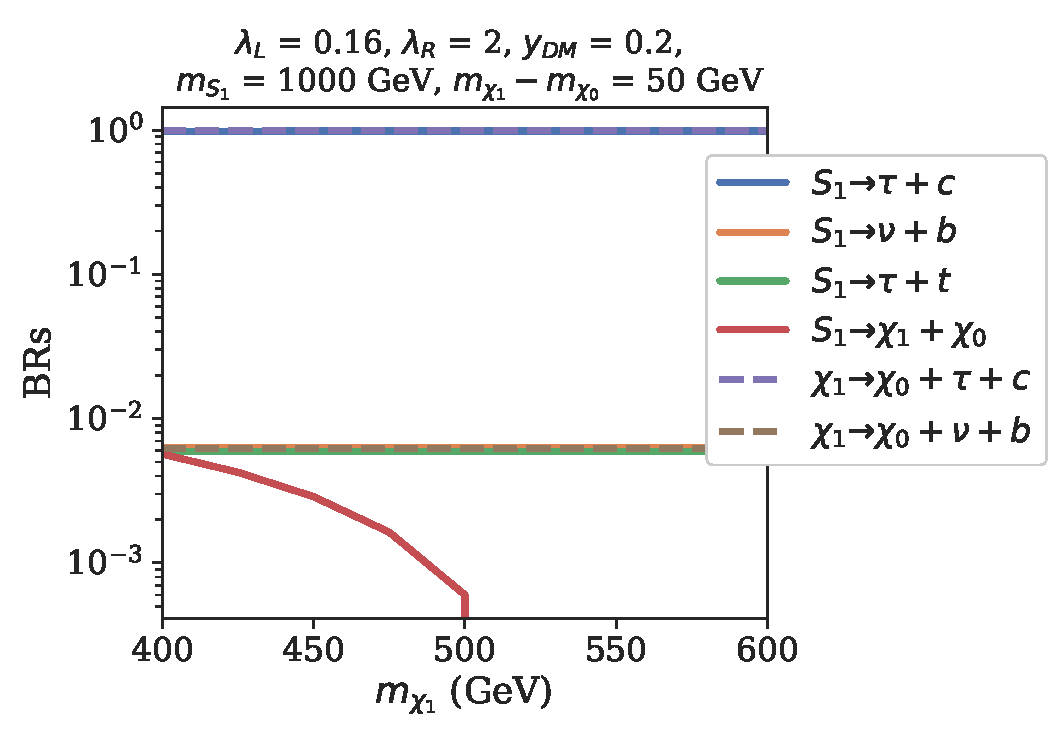
\includegraphics[width=0.5\textwidth]{figures/brsBM1.pdf}
	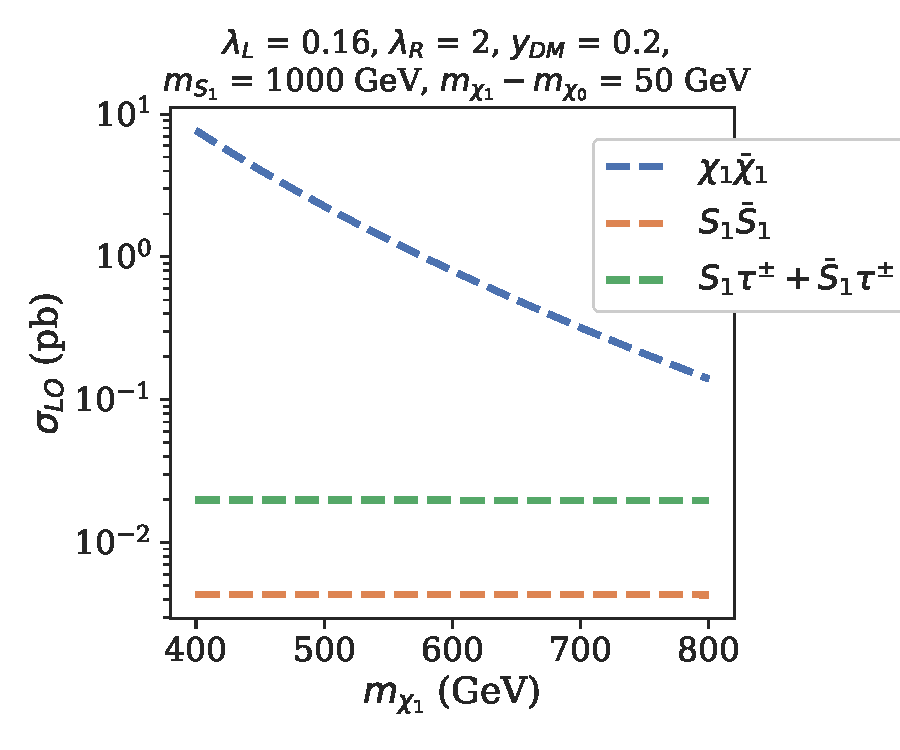
\includegraphics[width=0.45\textwidth]{figures/xsecsBM1.pdf}
	\caption{Branching ratios (left) and production cross-sections at the 13~TeV  LHC (right) for $S_1$ and $\chi_1$ as a function of the $\chi_1$ mass. The mass difference between $\chi_1$ and $\chi_0$ is kept as 50~GeV, $y_{\chi} = 0.2$ and all the other parameters correpond to the best fit benchmark model listed in Table~\ref{tab:benchmark_points}: $\lambda_L = 0.16, \lambda_R = 2.0$ and $m_{S_1} = 1$~TeV.
		\label{fig:xsecBRs}
	}
\end{figure}
%                                      \         |
%                                        \       |
%                                          \     |
%=====================





\subsection{Leptoquark searches}

\JZ{Under study by JB, GP, PP, JZ, AJ}

\subsubsection{LQ pair searches}

Pair production of LQs at the LHC proceeds via gauge couplings, as shown in the left panel of Fig~\ref{fig:LQvisible}.

%%%%%%%%%%%%%%%%%%%%%%%%%%%%%%%%%%%%%%%%%%%%%%%%%%%%%%%%%%%%%%%%%%%%%%%%%%%%%%%%%%%%%%%%%%%%%%%%%%%%%%%%%%%%%%
 \begin{figure}[!htp]
  \centering
  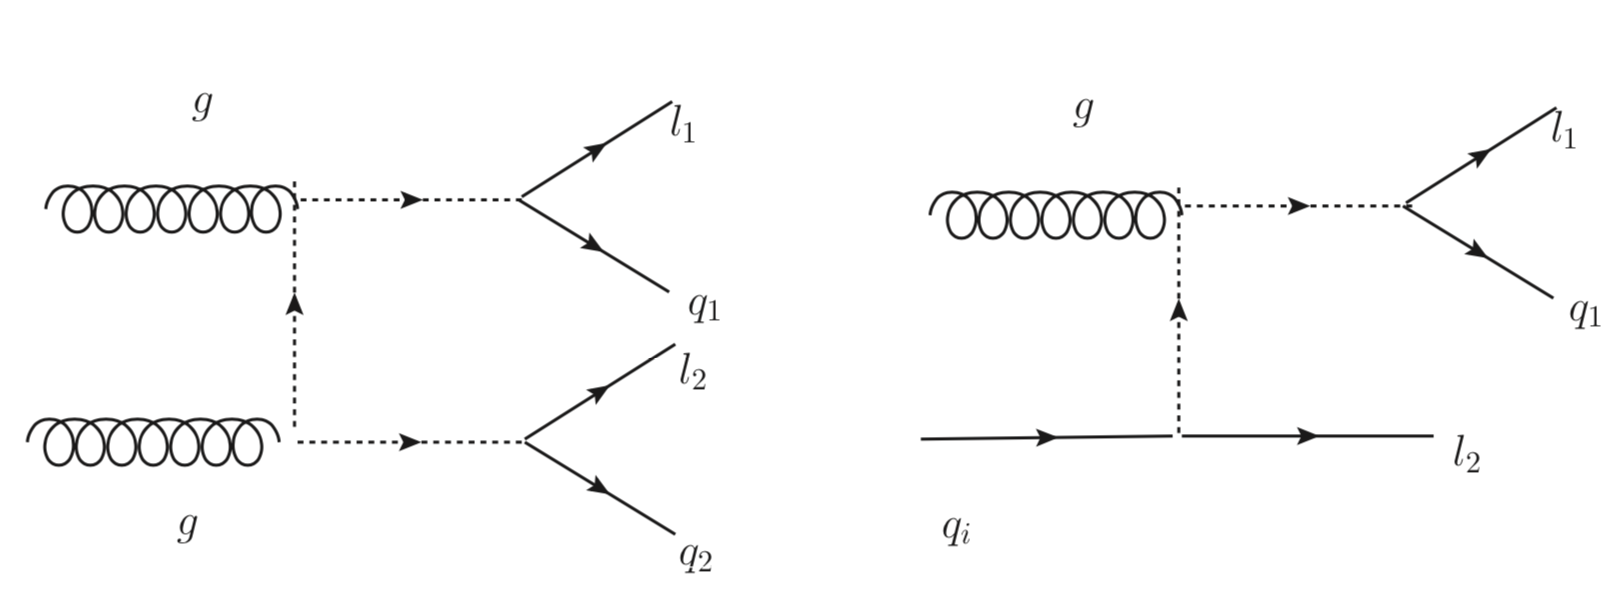
\includegraphics[width=0.5\textwidth]{./figures/LQ_visible.png} 
  \caption{\it Leptoquark production at the LHC: single (left) and double (right), considering visible decays.}
\label{fig:LQvisible}
\end{figure}
%%%%%%%%%%%%%%%%%%%%%%%%%%%%%%%%%%%%%%%%%%%%%%%%%%%%%%%%%%%%%%%%%%%%%%%%%%%%%%%%%%%%%%%%%%%%%%%%%%%%%%%%%%%%%%
Searches for visible decays of LQ pairs at ATLAS~\cite{Aad:2015caa,Aaboud:2019jcc,Aaboud:2019bye} and CMS~\cite{Sirunyan:2018nkj,Sirunyan:2018kzh,Sirunyan:2018vhk}, focus on both leptoquarks decaying in the same final state. In Ref.~\cite{Aaboud:2019bye} five different searches are described. The first one is a search for LQ decaying into the $b \tau b \tau$ final state, based on an existing di-Higgs search in the same final state~\cite{Aaboud:2018sfw}, albeit with different kinematics. The other four searches are reinterpretations of existing studies of supersymmetric particles: searches for stop pair production in the zero-lepton~\cite{Aaboud:2017ayj} and one-lepton channel~\cite{Aaboud:2017aeu} ($t \bar{t} +$ MET), stop decays into staus~\cite{Aaboud:2018kya} and a sbottom search~\cite{Aaboud:2017wqg} ($b\bar{b} + $ MET ). Among these searches, what is relevant for our model are the final states of $b \tau b \tau$, which correspond to the decay of both leptoquarks in the $t \tau$ final state, and the search for $b \bar{b} +$ MET  which covers the case where both leptoquarks decay into $b \nu$. For any choice of the coupling, and barring effects from the top mass, we would have that $BR (S_1 \to t \tau) \approx BR (S_1 \to b \nu$, in contrast to the ATLAS study where $BR(S_1 b \nu) = 1 - BR(S_1 \to t \tau)$ is assumed. Thus, in order to achieve an optimal coverage of the parameter space, one should also include the final state $b \nu t \tau$, which we dubbed the ``mixed" visible leptoquark search. We present in Fig~\ref{fig:LQpaircoverage} the corresponding branching ratios into $t \tau$ (solid red) and $b \nu$ (solid blue) for the scenario where only $\lambda_L$ is turned on, together with the reach in the $t \tau t \tau$ (dashed red), $b \nu b \nu$ (dashed blue) and our proposed search $t \tau b \nu$ (dashed green).
%%%%%%%%%%
 \begin{figure}[!htp]
  \centering
  \includegraphics[width=0.8\textwidth]{./figures/lq_exclusions_RD_compatible_plus_mixed.pdf} 
%  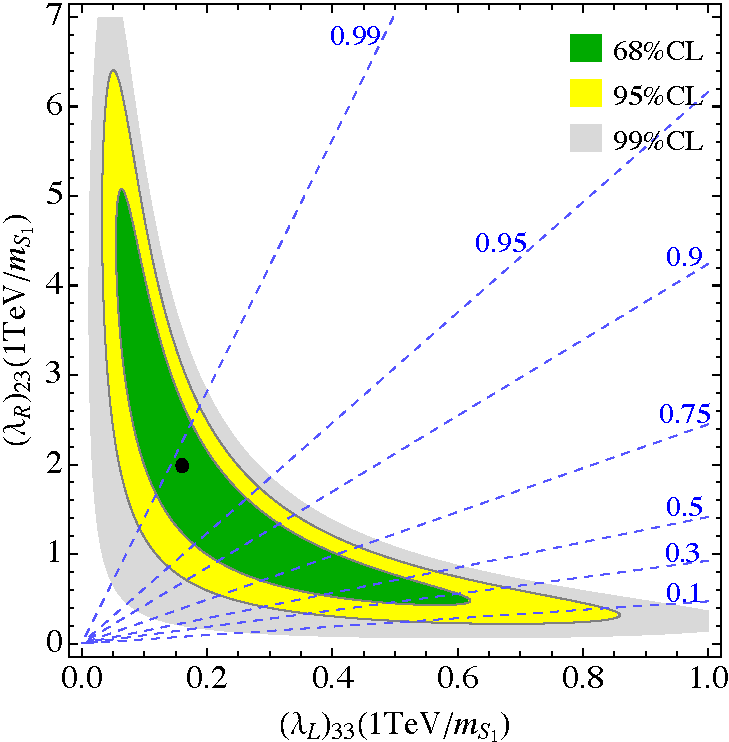
\includegraphics[width=0.44\textwidth]{./figures/FlavorFit_S1.pdf} 
  \caption{\it Coverage of the different LQ pair searches with decays into third generation fermions. We show in solid lines the branching ratio for the case where only $\lambda_L$ is non-zero, namely where the leptoquark decays exclusively into $b \nu$ (blue) and $t \tau$ (red). Note that both branching fractions should be equal if the top mass were negligible with respect to $m_{S_1}$. We also present in dashed lines the reach of the ATLAS search for $t \tau t \tau$ (red), $b \nu b \nu$ (blue), taken from~\cite{Aaboud:2019bye}, as well as our proposed search in the $t \tau b \nu$ channel (green). The latter final state provides the best coverage of the parameter space provided that $m_{S_1} \gtrsim$ 500 GeV. l}
\label{fig:LQpaircoverage}
\end{figure}
%%%%%%%%%%%

We thus see that above 500 GeV the mixed search has the best coverage, and thus we will adopt this search to carry out our projections for the HL-LHC~\footnote{\JZ{This last sentence is from Giacomo. I am not sure if for the proceedings we will do HL-LHC, but I agree with the philosophy of using only the best search for LQ pairs.}}. In view of these results we encourage the experimental collaborations to design a full-fledged analysis targeting the mixed decay. However it is clear from the fits to the charged-current flavor anomalies of Figure~\ref{fig:David} and from our benchmark points shown in Table~\ref{tab:benchmark_points} that the search based exclusively on the third generation final states is insufficient to cover the $\RD$-compatible parameter: since $\lambda_R$ is always larger than  $\lambda_L$,  $S_1$ decays predominantly into the $c \tau$ final state. Thus a search including this final state (in particular the $c \tau c \tau$ channel) would be needed. In view of the impressive results achieved in final states with two $c$-tagged quarks~\cite{} \JZ{Need citations from Giacomo}, this analysis should be feasible, however is outside the scope of this proceeding. \JZ{Does it mean that we want to do it for the paper?}.


\subsubsection{LQ associated production (with lepton and/or jet)}
\JZ{In charge: JZ, AB, DS, AJ} \\
A single leptoquark can also be produced in association with a SM fermion, as shown in the right panel of Fig~\ref{fig:LQvisible}. For our particular choice of couplings, we expect that one can have some sensitivity if this fermion is a charged lepton, hence if $l_2=e, \mu, \tau$.

\JZ{To the best of my understanding this is under study by David, Giacomo and others. At the current stage I would be happy to point out to their study within the same proceedings.}


\subsection{Dark matter (missing energy) searches}
\label{subsec:mjet}
Since the $\chi_1$ particle is the lightest new particle with non-trivial SM quantum numbers, its production is strongly constrained by LHC searches, and it can only be ``hidden" if $\chi_1$ and $\chi_0$ are close in mass. The LHC production is depicted in Fig.~\ref{fig:MonoJet}. The usual strategy against a compressed spectra is to boost the system with additional radiation, leading to the mono-X (typically jet) signals. 

%%%%%%%%%%%%%%%%%%%%%%%%%%%%%%%%%%%%%%%%%%%%%%%%%%%%%%%%%%%%%%%%%%%%%%%%%%%%%%%%%%%%%%%%%%%%%%%%%%%%%%%%%%%%%%
 \begin{figure}[!htp]
  \centering
  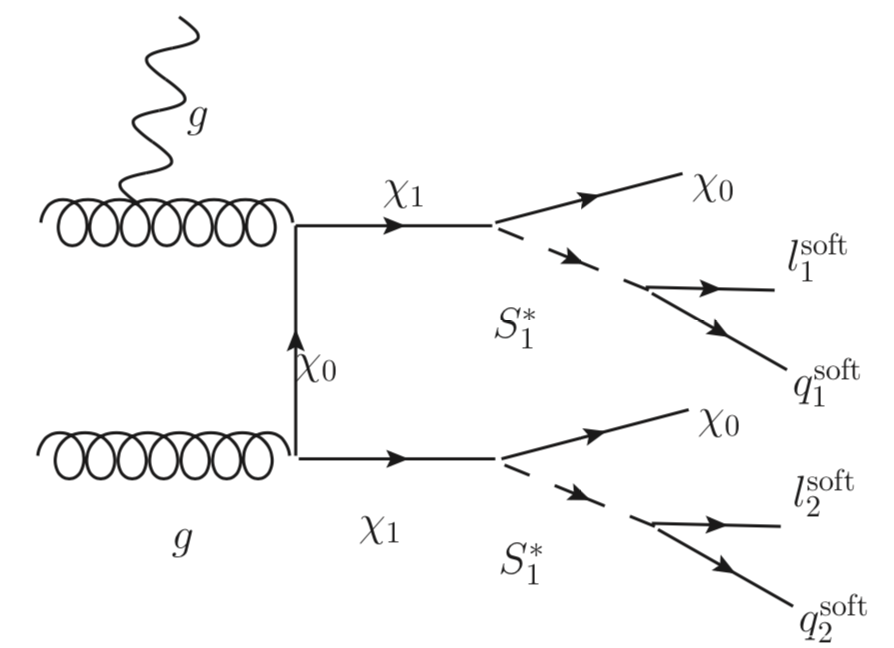
\includegraphics[width=0.5\textwidth]{./figures/MonoJet.png} 
  \caption{\it Monojet (plus soft leptons and quarks) signatures.}
\label{fig:MonoJet}
\end{figure}
%%%%%%%%%%%%%%%%%%%%%%%%%%%%%%%%%%%%%%%%%%%%%%%%%%%%%%%%%%%%%%%%%%%%%%%%%%%%%%%%%%%%%%%%%%%%%%%%%%%%%%%%%%%%%%

However, if the SM decay products in the $\chi_1 \to \chi_0$ are soft enough to be reconstructed (but probably not to triggered on) the LHC sensitivity gets greatly enhanced, as shown in e.g: ~\cite{Schwaller:2013baa} for MSSM electroweakinos and soft-leptons. However, the mass gap can be small enough such that the soft decay products fail to pass the reconstruction thresholds, in which case the pair production of $\chi$ particles can only be constrained by  mono-jet searches. We stress that this is an unavoidable bound, that, for a given $\Delta$, sets a lower mass on the dark sector masses. We will thus ignore here the MET searches that also include resolved (soft or hard) leptons. \JZ{This last sentence needs to be revisited depending on what is available in MadAnalysis, CheckMATE or similar}.



%=====================
%    \                                           |
%      \                                         |
%        \                                       |
\begin{figure}[!h]
	\centering
	\includegraphics[width=0.6\textwidth]{figures/T2bb_exclusion.pdf}
	\caption{Region in the $m_{\chi_1} - m_{\chi_0}$ vs $m_{\chi_1}$ plane excluded by LHC MET searches. The remaining model parameters are $y_{\chi} = 0.2$, $\lambda_L = 0.16, \lambda_R = 2.0$ and $m_{S_1} = 1$~TeV. The shaded region corresponds to the parameter space excluded by ATLAS and CMS searches for final states containing one or more b-jets and missing energy. {\it The signal efficiencies are assumed to be the same as for sbottom pair production followed by $\tilde{b} \to b + \chi_1^0$ decays. We do not take into account possible effects due to the 3-body decay of $\chi_1$ ($\chi_1 \to b + \chi_0 + \nu$).}
		\label{fig:T2bbexcl}
	}
\end{figure}
%                                      \         |
%                                        \       |
%                                          \     |
%=====================



\subsection{Resonant lepto-quark + MET search}

\JZ{Benj wants to recast the CMS study, \cite{Sirunyan:2018xtm}. AJ will help him. }.


%
%%%%%%%%%%%%%%%%%%%%%%%%%%%%%%%%%%%%%%%%%%%%%%%%%%%%%%%%%%%%%%%%%%%%%%%%%%%%%%%%%%%%%%%%%%%%%%%%%%%%%%%%%%%%%%%
% \begin{figure}
%  \centering
%  \includegraphics[width=0.75\textwidth]{plot.pdf} 
%  \caption{\it Abstract text.}
%\label{fig:fig}
%\end{figure}
% 
%%%%%%%%%%%%%%%%%%%%%%%%%%%%%%%%%%%%%%%%%%%%%%%%%%%%%%%%%%%%%%%%%%%%%%%%%%%%%%%%%%%%%%%%%%%%%%%%%%%%%%%%%%%%%%%
 

\section{CONCLUSIONS}
The charged-current flavor anomalies hint at the present of leptoquarks near or at the TeV scale. Here we have studied the connection between these models and dark matter, which necessarily requires to add new particles and couplings. Employing a simplified model with only 6 parameters we have scanned the parameter space vis-a-vis the aformentioned flavor anomalies, relic density, direct detection and LHC constraints.

We have seen that when taken all these constraints simultaneously one is left with two possible scenarios: either the dark sector couples to the leptoquark mediator with a similar strength than the one required from taking the $\RD$ anomaly at face-value, which then implies a traditional freeze-out scenario to account for the current abundance of dark matter, or the leptoquark couples faintly to the dark sector, which in turn implies that the dark matter abundance arises from the conversion-driven freeze-out (co-scattering) mechanism.  In the second scenario the leptoquark branching fraction into the dark sector is negligible, and thus the phenomenology will consist of seemingly disconnected leptoquark ``anomaly-inspired" and traditional missing energy + X signatures. In the latter case, depending on the ``compression" between the dark sector particles, one can resolve the leptons and quarks from the $S_1 \to \chi_1 \chi_0 \to l q \chi_0 \chi_0$ decay chain, which would then allow to establish a firm connection between both new physics signals. In the case where the branching fraction into the dark sector is non-negligilbe, then the strongest indication of the leptoquark-dark matter connection is through the pair production of leptoquarks with one decaying into the dark sector and another one into hard leptons and quarks. Since this search is only being conducted currently by the CMS collaboration, we urge ATLAS to undertake this key study for a comprehensive dark matter program going beyond the mere annihilation into singlet final states.

Along this work we have pointed out the existence of two important holes in the campaign to optimal cover the leptoqaurk parameter space. On one side we have noted that for leptoquarks decaying into the third generation fermions (almost) exclusively, a search in the $b \nu t \tau$ should be added to the existing ones looking into $b \nu b \nu$ and $t \tau t \tau$, where one can benefit from a larger branching fraction, and devise cuts to keep the background under control, which we have demonstrated with a simple analysis. On the other side, noting that the solutions to the $\RD$ anomalies involve larger couplings connecting second generation quarks with third generation leptons, we advocate to study the $c \tau c \tau$ final state, and if possible and depending on the $c$-tagging efficiencies, also include the mixed cases, e.g $c \tau t \tau$ or $b \nu c \tau$ final states.  

%.... \JZ{SOMETHING}. We thus encourage the LHC collaborations to ... \JZ{DO A NEW SEARCH THAT MIGHT BE IMPORTANT / CONVINCE ATLAS OF DOING THE LQ RESONANT + MET STUDY}. 

Our results show that... \JZ{describe final parameter space allowed}.
Naively rescaling our results for the HL-LHC we find that (\JZ{hopefully}) the parameter space favored by the flavor anomalies will be fully covered with just 1000 fb$^{-1}$ of data. \JZ{Maybe we will leave the projections for the paper?}


\section*{ACKNOWLEDGEMENTS}
We would like to thank AAA and BBB for useful discussions.
The work of XXX was supported (in part) by ....



\appendix
\section{Appendix A}



\bibliography{RDM_LH2019}

\end{document}
